\subsection{Geometric interpretation of Gauss curvature}
Assume \(K_p\neq 0\).
\begin{enumerate}[(a)]
    \item \(p\in S\), \(U\) is a neighborhood of \(p\). \(N\colon
          S\to \mathbb{S}^2\) is the Gauss map.
          \begin{center}
              \tikzset{every picture/.style={line width=0.75pt}} %set default line width to 0.75pt        
              \begin{tikzpicture}[x=0.75pt,y=0.75pt,yscale=-0.9,xscale=0.9]
                  %uncomment if require: \path (0,300); %set diagram left start at 0, and has height of 300

                  %Curve Lines [id:da6642321506777753] 
                  \draw    (69,92) .. controls (109,62) and (234.4,104.
                  5) .. (274.4,74.5) ;
                  %Curve Lines [id:da5984856894036306] 
                  \draw    (38.4,193.5) .. controls (44.4,143.5) and (75.4,
                  124.5) .. (69,92) ;
                  %Curve Lines [id:da6894898997393564] 
                  \draw    (38.4,193.5) .. controls (78.4,163.5) and (203.8,
                  206) .. (243.8,176) ;
                  %Curve Lines [id:da28193586114058156] 
                  \draw    (243.8,176) .. controls (249.8,126) and (280.8,
                  107) .. (274.4,74.5) ;
                  %Shape: Circle [id:dp2732770518905623] 
                  \draw   (135.2,137.2) .. controls (135.2,123.39) and (146.
                  39,112.2) .. (160.2,112.2) .. controls (174.01,112.2) and 
                  (185.2,123.39) .. (185.2,137.2) .. controls (185.2,151.
                  01) and (174.01,162.2) .. (160.2,162.2) .. controls (146.
                  39,162.2) and (135.2,151.01) .. (135.2,137.2) -- cycle ;
                  %Shape: Circle [id:dp5729113128085532] 
                  \draw  [fill={rgb, 255:red, 0; green, 0; blue, 0 }  ,fill
                   opacity=1 ] (158,135) .. controls (158,133.78) and (158.
                   98,132.8) .. (160.2,132.8) .. controls (161.41,132.8) 
                   and (162.4,133.78) .. (162.4,135) .. controls (162.4,136.
                   22) and (161.41,137.2) .. (160.2,137.2) .. controls (158.
                   98,137.2) and (158,136.22) .. (158,135) -- cycle ;
                  %Shape: Circle [id:dp4525846429117777] 
                  \draw   (468,109.75) .. controls (468,70.4) and (499.9,38.
                  5) .. (539.25,38.5) .. controls (578.6,38.5) and (610.5,
                  70.4) .. (610.5,109.75) .. controls (610.5,149.1) and 
                  (578.6,181) .. (539.25,181) .. controls (499.9,181) and 
                  (468,149.1) .. (468,109.75) -- cycle ;
                  %Shape: Arc [id:dp8314742253507434] 
                  \draw  [draw opacity=0] (608.75,124.26) .. controls (569.
                  98,163.03) and (507.53,163.45) .. (469.27,125.18) -- (539.
                  47,54.98) -- cycle ; \draw   (608.75,124.26) .. controls 
                  (569.98,163.03) and (507.53,163.45) .. (469.27,125.18) ;
                  %Shape: Arc [id:dp9893025234051245] 
                  \draw  [draw opacity=0][dash pattern={on 0.84pt off 2.51pt}] (469.27,125.18) .. controls (508.04,86.41) and (570.49,86) .. (608.75,124.26) -- (538.55,194.46) -- cycle ; \draw  [dash pattern={on 0.84pt off 2.51pt}] (469.27,125.18) .. controls (508.04,86.41) and (570.49,86) .. (608.75,124.26) ;
                  %Shape: Arc [id:dp816831718894679] 
                  \draw  [draw opacity=0] (586.34,57.22) .. controls (555.97,71.4) and (522.37,72.11) .. (494.62,56.03) -- (557.97,-53.27) -- cycle ; \draw   (586.34,57.22) .. controls (555.97,71.4) and (522.37,72.11) .. (494.62,56.03) ;
                  %Shape: Arc [id:dp9897455191573623] 
                  \draw  [draw opacity=0][dash pattern={on 0.84pt off 2.51pt}] (494.62,56.19) .. controls (524.97,41.96) and (558.56,41.18) .. (586.34,57.22) -- (523.18,166.63) -- cycle ; \draw  [dash pattern={on 0.84pt off 2.51pt}] (494.62,56.19) .. controls (524.97,41.96) and (558.56,41.18) .. (586.34,57.22) ;
                  %Shape: Circle [id:dp6595482110117465] 
                  \draw  [fill={rgb, 255:red, 0; green, 0; blue, 0 }  ,fill opacity=1 ] (539.25,38.5) .. controls (539.25,37.28) and (540.23,36.3) .. (541.45,36.3) .. controls (542.66,36.3) and (543.65,37.28) .. (543.65,38.5) .. controls (543.65,39.72) and (542.66,40.7) .. (541.45,40.7) .. controls (540.23,40.7) and (539.25,39.72) .. (539.25,38.5) -- cycle ;
                  %Straight Lines [id:da12514301449881793] 
                  \draw    (315,131) -- (428.4,127.56) ;
                  \draw [shift={(430.4,127.5)}, rotate = 178.26] [color={rgb, 255:red, 0; green, 0; blue, 0 }  ][line width=0.75]    (10.93,-3.29) .. controls (6.95,-1.4) and (3.31,-0.3) .. (0,0) .. controls (3.31,0.3) and (6.95,1.4) .. (10.93,3.29)   ;

                  % Text Node
                  \draw (155,135.4) node [anchor=north west][inner sep=0.75pt]    {$p$};
                  % Text Node
                  \draw (195,102.4) node [anchor=north west][inner sep=0.75pt]    {$U$};
                  % Text Node
                  \draw (272,56.4) node [anchor=north west][inner sep=0.75pt]    {$S$};
                  % Text Node
                  \draw (518,13.4) node [anchor=north west][inner sep=0.75pt]    {$N( p)$};
                  % Text Node
                  \draw (624,38.4) node [anchor=north west][inner sep=0.75pt]    {$\mathbb{S}^{2}$};
                  % Text Node
                  \draw (364,102.4) node [anchor=north west][inner sep=0.75pt]    {$N$};
              \end{tikzpicture}
          \end{center}
          Let \(A\)= Area of \(U\), \(\var{A}\)= Area of \(N(U)\),
          then 
          \[
            |K(p)|=\lim_{A\to 0}\frac{\bar{A}}{A}.\tag{1}  
          \]
          \item \(p\in T_p S\)=tangent plane \(\simeq \mathbb{R}^2\). 
          Consider a circle of radius \(r\) in \(T_p S\) and a ``circle''
          of radius \(r\) on \(S\).
          \begin{center}
            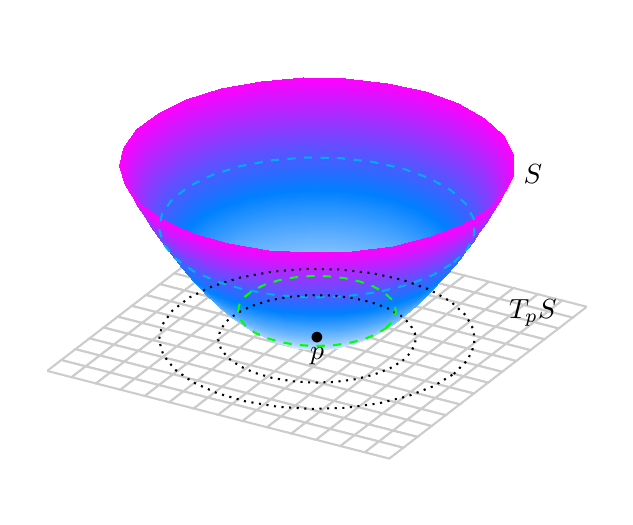
\begin{tikzpicture}
                \begin{axis}[xticklabels={,,},%不显示x坐标轴数字
                    yticklabels={,,},
                    zticklabels={,,},
                    axis line style={draw=none},%不显示坐标轴
                    tick style={draw=none},
                    colormap/cool,
                    view={30}{40}
                ]
                \addplot3 [
                    surf,
                    domain=-1:1, domain y=-1:1,
                    samples=15, samples y=15,
                ] ({x},{y},{0});
                \addplot3[
                    surf,
                    shader=interp,
                    z buffer=sort,
                    domain=0:360, domain y=0:1,
                    samples=30, samples y=30,
                    variable=\u, variable y=\v,
                    ]({v*cos(u)},{v*sin(u)},{v*v});
                    \node[text=black] at (0,0,-0.1) {\(p\)};
                    \node at (0,0,0) {\(\bullet\)};
                    \node[text=black] at (0.8,0.8,0) {\(T_p S\)};
                    \node[text=black] at (0.8,0.8,0.8) {\(S\)};
                \addplot3 [
                    black,
                    dotted,
                    domain=0:360,
                    samples=30,
                    samples y=1%防止曲线闭合
                ]({0.8*cos(x)},{0.8*sin(x)},0);
                \addplot3 [
                    cyan,
                    dashed,
                    domain=0:360,
                    samples=30,
                    samples y=1%防止曲线闭合
                ]({0.8*cos(x)},{0.8*sin(x)},{0.64});
                \addplot3 [
                    black,
                    dotted,
                    domain=0:360,
                    samples=30,
                    samples y=1%防止曲线闭合
                ]({0.5*cos(x)},{0.5*sin(x)},0);
                \addplot3 [
                    green,
                    dashed,
                    domain=0:360,
                    samples=30,
                    samples y=1%防止曲线闭合
                ]({0.4*cos(x)},{0.4*sin(x)},{0.16});
                \end{axis} 
            \end{tikzpicture}
          \end{center}
          Then
          \[\label{geometric meaning curvature 2}
            K(p)=\lim_{r\to 0}3\frac{2\pi r-c(r)}{\pi r^3},\tag{2}  
          \]
          where \(c(r)\)= circumference of the circle of radius \(r\)
          on \(S\).
          \item Consider a disk around \(p\) of radius \(r\) in \(T_p S\). 
          Also consider a ``disk'' around \(p\) of radius \(r\) on 
          \(S\).
          \[\label{geometric meaning curvature 3}
            K(p)=\lim_{r\to 0} 12\frac{\pi r^2-A(r)}{\pi r^4},\tag{3}
          \]
          where \(A(r)\)= Area of disk on \(S\).
\end{enumerate}
\begin{remark}
    From expression of \cref{geometric meaning curvature 2} 
    and \cref{geometric meaning curvature 3}, one can prove 
    them by considering the Taylor's expansion of \(c(r)\)
    and \(A(r)\). The proof of these two facts will be postponed
     after we step into intrinsic geometry.(Need Taylor's expansion
      of metric tensor)
\end{remark}
\begin{proof}
    Let \(F(u,v)\) be the local parametrization on \(U\).
    \[
        \Rightarrow Area(U)=\iint_{F^{-1}(U)}\left|
            F_u\wedge F_v
        \right| \dd u\dd v,
    \]
    then \(T_{N(p)}N(U)=\Span\{N_u,N_v\}\),
    \[
        \bar{A}=\iint_{F^{-1}(U)} \left|N_u\wedge N_v\right|\dd u
        \dd v.
    \]
    \underline{Recall}: \(dN\begin{pmatrix}
        F_u\\
        F_v
    \end{pmatrix}=\begin{pmatrix}
        N_u\\N_v
    \end{pmatrix}=A\begin{pmatrix}
        F_u\\
        F_v
    \end{pmatrix}\), where \(A\) is the Weingarten matrix.
    \[
        \Rightarrow \left|
            N_u \wedge N_v
        \right|=\left|\det A\right|\left|
            F_u\wedge F_v
        \right|=|K|\left|
            F_u\wedge F_v
        \right|.
    \]
    \begin{align*}
        \frac{\bar{A}}{A}&=\frac{\iint |K|\left|
            F_u\wedge F_v
        \right|\dd u \dd v}{\iint \left|
            F_u\wedge F_v
        \right|\dd u\dd v}\\
        &=\frac{|K(q)|\left|
            F_u\wedge F_v
        \right|(q)Area(F^{-1}(U))}{\left|
            F_u\wedge F_v
        \right|(\bar{q})Area(F^{-1}(U))}\quad (\text{Middle value theorem}).
    \end{align*}
    As \(A\to 0\), \(q\to p\), \(\bar{q}\to p\),
    \[\Rightarrow |K(p)|=\lim_{A\to 0}\frac{\bar{A}}{A}.\]
\end{proof}
\section{More Examples}
\begin{exercise}
    Graph \(z=h(x,y)\)= \(S\). 
\end{exercise}
(\underline{Recall}: For a regular surface, by the implicit (inverse) 
function theorem, it can be written as a graph locally.)

In the HW 8, you may have computed 
\[
    I=\left(1+h_x^2\right)\dd x^2+2h_x h_y\dd x\dd y+(1+h_y^2)\dd y^2
\]
\[
    \II =\frac{h_{xx}}{\sqrt{1+\left|\nabla h\right|_{\mathbb{R}^2}^2}}
    \dd x^2 +2 \frac{h_{x}h_y}{\sqrt{1+\left|\nabla h
    \right|^2}}\dd x\dd y+\frac{h_{yy}}{\sqrt{1+\left|
        \nabla h\right|^2}}\dd y^2.
\]
\[
N=\frac{\left(-h_x,-h_y,1\right)}{\sqrt{1+\left|
    \nabla h\right|^2}}.    
\]
\[
    K=\frac{h_{xx}h_{yy}-h_{xy}^2}{\left(1+\left|
        \nabla h\right|^2\right)^2}=\frac{\det \nabla^2h}{\left(1+\left|
            \nabla h\right|^2\right)^2}.
\]
\[
    2H=\frac{(1+h_x^2)h_{yy}-2 h_x h_y h_{xy}+(1+h_y^2)h_{xx}}{
        \left(1+\left|
            \nabla h\right|^2\right)^{\frac{3}{2}}
    }    .
    \footnotemark
\]
\footnotetext{A basic observation one should make is how \(K\) and
\(H\) depend on the \engordnumber{2} derivative of \(h\).}
Note that the last term equals \[
    \mathrm{div}_{\mathbb{R}^2}\left(\frac{\nabla h}{
        \sqrt{1+\left|
            \nabla h\right|^2}
    }\right)
    =
    \sum_{i,j=1}^2 L^{ij}\left(\nabla f\right)\nabla_i\nabla_j h,
\]
where \[
    L^{ij}\left(\nabla f\right)=\frac{1}{\sqrt{1+\left|
        \nabla h\right|^2}}\left(\delta_{ij}-
        \frac{\nabla_i h\nabla_j h}{1+\left|
            \nabla h\right|^2}\right)    .
\]
Let \(p\in S\), and assume \(p\) is the origin in \(\mathbb{R}^3\),
 and \(N\) agrees with the unit normal of \(z\)-axis
 \[
    h_x=h_y=0\text{ at p}.   
 \]
 \[
    e=h_{xx}(0,0), f=h_{xy}(0,0), g=h_{yy}(0,0).   
 \]
 Hessian of \(h\) at \(p\) is 
 \[
    \begin{pmatrix}
        h_{xx}(0,0)& h_{xy}(0,0)\\
        h_{yx}(0,0)&h_{yy}(0,0)
    \end{pmatrix} .  
 \]
 Hence, at \(p\)
 \[
    \II=\mathrm{Hess}~h.   
 \]
 Moreover, at \(p\)
 \[
    \partial H=\delta h.
 \]
 As an application, we give a geometric interpretation of the Dupin
 indicatrix.
 \underline{Claim}: If \(p\in S\) is not a planar point, consider the 
 intersection of a plane parallel to \(T_p S\) with \(S\), and the plane
  is close enough to \(T_p S\), then the obtained curve is approximated
   by the Dupin indicatrix.
\begin{proof}
    Since we only care about local behavior at \(p\), W.L.O.G assume
     near \(p\), the surface is parametrized by the graph \(z=h(x,y)\),
     such that \(p\) is the origin and \(z\)-axis is the normal direction 
      and \(x\)-axis, \(y\)-axis are principal directions.
      Let the intersection curve be \(h(x,y)=\epsilon\), for sufficiently
      small \(\epsilon\). Consider the Tayler's expansion of 
      \(h(x,y)\) at \(p\)
      \begin{align*}
        h(x,y)=&h(0,0)+h_x(0,0)x+h_y(0,0)y\\
        &+\frac{1}{2}\left(
            h_{xx}(0,0)x^2+\underbrace{2h_{xy}(0,0)}_{
                =0\text{(principal direction)}
            }xy+h_yy(0,0)y^2
        \right)\\
        &+\text{Remainder}\\
        =&\frac{1}{2}\begin{pmatrix}
            x&y
        \end{pmatrix}
        \begin{pmatrix}
            h_{xx}(0,0)&0\\
            0&h_{yy}(0,0)
        \end{pmatrix}
        \begin{pmatrix}
            x\\
            y
        \end{pmatrix}+\text{Remainder},
      \end{align*}
\end{proof}
where 
\[
    \lim_{(x,y)\to (0,0)}    \frac{\text{Remainder}}{x^2+y^2}=0.
\]
Hence, the intersection curve is given by 
\[
    \frac{1}{2}\left(h_{xx}(0,0)x^2+h_{yy}(0,0)y^2\right)+R=\epsilon.    
\]
Note: in the \engordnumber{2} fundamental form\(II\) \(f=0\), 
and in the  \engordnumber{1} fundamental form \(I\) \(F=0\),
then at \(p\) one has 
\[
    \begin{cases}
        k_1=\frac{e}{E}=h_{xx}(0,0)\\
        k_2=\frac{g}{G}=h_{yy}(0,0)
    \end{cases}    
\]
using \(k_i=H\pm\sqrt{H^2-K}\). Then, \(k_1x^2+k_2y^2=2\epsilon\)
can be viewed as the \engordnumber{1} order approximation of the 
intersection curve. Renormalized it, then 
\[k_1 \bar{x}^2+k_2\bar{y}^2=1.\]
is just the Dupin indicatrix.
